\section{Implementazione} \label{sec:tecn}

\subsection{Architettura hardware} \label{subsec:hard}
I terapisti hanno bisogno di poter vedere quello che il bambino compie durante l'esperienza di gioco per cui abbiamo la necessità di replicare lo schermo dello smartphone su pc: questo verrà effettuato con l'uso di Google Chromecast.
\vspace{70pt}
\begin{figure}[htbp]
\centering
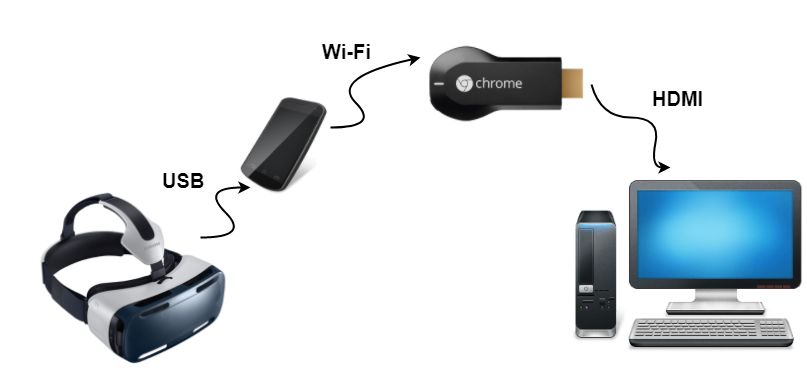
\includegraphics[width=\textwidth]{Images/hardware}
\caption{Architettura hardware}
\label{fig:hardware}
\end{figure}
\clearpage

\subsection{Architettura software} \label{subsec:soft}
L'architettura software prevede la comunicazione di tre moduli principali: l'applicazione \acs{gea}, con cui il terapista (nella scelta iniziale del livello di difficoltà) comunica, che è collegata al programma di gestione di orientamento visivo (necessario per captare i movimenti e il focus del bambino) del \acs{vr} e che trasferisce i dati al \acs{pc} del terapista che può quindi monitorare l'avanzamento del gioco e dare perciò eventuali suggerimenti al paziente.
\vspace{70pt}
\begin{figure}[htbp]
\centering
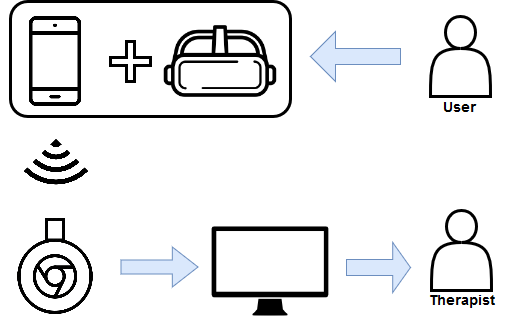
\includegraphics[width=\textwidth]{Images/software}
\caption{Architettura software}
\label{fig:software}
\end{figure}
\clearpage

\subsection{Linguaggi di programmazione e software utilizzati} \label{subsec:ling}
Di seguito vengono elencati i linguaggi di programmazione e i software utilizzati per sviluppare l'applicazione in realtà virtuale \acs{gea}.
\subsubsection{Linguaggi di programmazione}
\begin{itemize}
	\item \acs{html}
	\item \acs{css}
	\item JavaScript
	\item A-Frame
	\item \acs{php}
	\item JQuery
\end{itemize}
\subsubsection{Software}
\begin{itemize}
	\item Brackets
	\item AlterVista
	\item FileZilla
	\item Imgur
\end{itemize}